\documentclass[]{article}
\usepackage{amsmath}
\usepackage{amssymb}
\usepackage{amsthm}
\usepackage{listings}
\usepackage{multirow}
\usepackage{tikz}
\usetikzlibrary{arrows,automata}
\begin{document}

\title{COMS W3261 \\ Computer Science Theory \\ Lecture 2\\ Finite Automata}
\author{Alexander Roth}
\date{2014-09-08}
\maketitle

\section*{Outline}
  \begin{itemize}
    \item Our languages odyssey
    \item Deterministic finite automata
    \item Examples of DFAs
    \item Nondeterministic finite automata
    \item Equivalence of DFAs and NFAs: the Subset Construction
    \item Bad Case for the Subset Construction
  \end{itemize}

\section{Our Languages Odyssey}
  \begin{itemize}
    \item In this course we will study the following classes of languages in the
    Chomsky hierarchy:
      \begin{itemize}
        \item The regular languages
        \item The context-free languages
        \item The recursive languages
        \item The recursively enumerable languages
      \end{itemize}
    \item We will discover that this is a proper hierarchy of languages.
  \end{itemize}
  \begin{description}
    \item[Regular Languages] Can be described using Finite Automata and
    Regular Expressions
    \item[Context-Free Grammars] Can be used to construct Regular Languages.
    \item[Algorithm] A Turing machine that halts on all inputs.
    \item[Recursively Enumerable] Does not halt on all inputs.
    \item[All Languages] What do you think? What kind of infinite is there?
  \end{description}
  If we look at any programming language, there are only a countably infinite
  number of programs; however, there are uncountably infinite languages. Thus,
  we reach a boundary of computing.

\section{Deterministic Finite Automata}
  \begin{itemize}
    \item A deterministic finite automation (DFA) is one of the simplest
    models of computation.
    \item A DFA defines a regular language.
    \item A DFA has five components:
      \begin{enumerate}
        \item A finite set of states $Q$.
        \item An input alphabet consisting of a finite set of symbols
        $\Sigma$.
        \item A transition function $\delta$ that maps $Q \times \Sigma$ to
        $Q$.\\
        This transition function can be represented by a transition diagram in
        which the nodes are labeled by states and arcs by symbols.
        \item A start state which is one of the states in $Q$.
        \item A set of final (or accepting) states $F$ that is a subset
        (possibly empty) of $Q$.
      \end{enumerate}
    \item A DFA accepts an input string $x$ if and only if there is a sequence
    of transitions from the initial state to a final state that spells out
    $x$.
    \item $L(D)$, the language defined by a DFA $D$, is the set of strings
    accepted by $D$.
    \item A language accepted by a DFA is called a \emph{regular language}.
  \end{itemize}
  We can imagine a Finite Automata as a circuit, which contains an input tape,
  with a read head and an input/output system. The machine starts in one state
  \texttt{A}, and moves along the tape. It begins in an initial condition, and
  then it makes a sequence of 0 or more moves until it reaches the final
  state, where it then says it \emph{accepts} the final state.

    \[ D = (Q, \Sigma, \delta, q_0, F) \]

  \begin{itemize}
    \item $D$ is the DFA.
    \item $Q$ is the finite set of states.
    \item $\Sigma$ is the input alphabet.
    \item $\delta$ is the transition function.
    \item $q_0$ is the start state.
    \item $F$ is the set of final states $F \subseteq Q$.
  \end{itemize}

    \[ \hat{\delta}: Q \times \Sigma^* \rightarrow Q \]

  where $\delta$ is $Q \times \Sigma \rightarrow Q$, that is the transition
  function that maps the alphabet to the finite state machine. \\
  \indent ``For every state and for every input symbol, there is a state it
  maps too.'' Everything need to be completely specified.

\section{Example 1: DFA for All Strings of 0's and 1's With an Even Number of
0's}
  \begin{itemize}
    \item Consider the following DFA $D$ with:
      \begin{enumerate}
        \item The finite set of states $Q = \{ \texttt{A, B} \}$
        \item The input alphabet $\Sigma = \{ \texttt{0, 1} \}$
        \item The transition function $\delta$ as represented by the following
        transition table:

          \begin{tabular}{|c|c|c|}
            \hline
            State & \multicolumn{2}{|c|}{Input Symbol} \\ \cline{2-3}
                  & \texttt{0} & \texttt{1} \\ \hline
            \texttt{A} & \texttt{B} & \texttt{A} \\ \hline
            \texttt{B} & \texttt{A} & \texttt{B} \\ \hline
          \end{tabular}

        \item Start state \texttt{A}
        \item The set of final states $F = \{ \texttt{A} \}$
      \end{enumerate}
    \item Given the input string \texttt{10101}, $D$ makes the following
    sequence of transitions started off in its start state \{\texttt{A}\}:\\
    \verb|  1   0   1   0   1  |\\
    \verb|A   A   B   B   A   A| \\
    The sequence of transitions take $D$ from its start state \texttt{A} to
    the final state \texttt{B}. Thus, the input \texttt{0010} is accepted by
    $D$
    \item Given the input string \texttt{101}, $D$ makes the following
    transitions started off in its initial start state \texttt{A}:\\
    \verb|  1   0   1  | \\
    \verb|A   A   B   B| \\
    This sequence of transitions takes $D$ from its start state \texttt{A} to
    the nonfinal state \texttt{B}. Therefore, the input \texttt{101} is not
    accepted by $D$.
    \item The language defined by $D$ is the set of all strings of 0's and 1's
    having an even number of 0's.
  \end{itemize}
  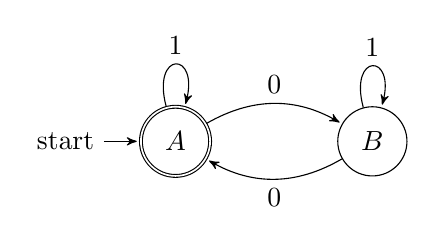
\begin{tikzpicture}[>=stealth',shorten >=1pt,auto,node distance=2.5cm]
    \node[initial,state,accepting] (A)              {$A$};
    \node[state]         (B) [right of=A] {$B$};

    \path[->] (A) edge [loop above] node  {1}   (A);
    \path[->] (A) edge [bend left] node  {0}   (B);
    \path[->] (B) edge [bend left] node {0}  (A);
    \path[->] (B) edge [loop above] node {1} (B);
  \end{tikzpicture}
  $L = \{ \, w | \, w \, \text{is a string of 0's and 1's with an even number of 0's} \, \}$

\section{Example 2: DFA for Binary Numbers Divisible by 3}
  \begin{itemize}
    \item We want a DFA to recognize all strings of 0's and 1's representing
    binary numbers divisible by three. We assume the empty string represents
    0, 0 represents 0, 1 represents 1, 00 represents 0, 01 represents 1, 10
    represents 2, 11 represents 3, and so on.
    \item Consider the following DFA $D$ with:
      \begin{enumerate}
        \item The finite set of states $Q = \{ \texttt{A, B, C} \}$
        \item The input alphabet $\Sigma = \{ \texttt{0, 1} \}$
        \item The transition function $\delta$ as represented by the following
        transition table:

          \begin{tabular}{|c|c|c|}
            \hline
            State & \multicolumn{2}{|c|}{Input Symbol} \\ \cline{2-3}
                  & \texttt{0} & \texttt{1} \\ \hline
            \texttt{A} & \texttt{A} & \texttt{B} \\ \hline
            \texttt{B} & \texttt{C} & \texttt{A} \\ \hline
            \texttt{C} & \texttt{B} & \texttt{C} \\ \hline
          \end{tabular}
        \item Start state \texttt{A}
        \item The set of final states $F = \{ \texttt{A} \}$
      \end{enumerate}
    \item State \texttt{A} represents all prefixes of binary strings that are
    congruent to 0 mod 3, state \texttt{B} all prefixes congruent to 1 mode 3,
    and state \texttt{C} all prefixes congruent to 2 mod 3.
    \item Given the input string \texttt{1001}, $D$ makes the following
    transitions started off in its start state \texttt{A}:\\
    \verb|  1   0   0   1   | \\
    \verb|A   B   C   B   A | \\
    In this sequence of transitions $D$ goes from its start state \texttt{A}.
    Thus, the binary input \texttt{1001}, which represents 9, is accepted by
    $D$.
  \end{itemize}

    \[ L = \{ \Sigma, 0, 11, 110, \ldots \} \]

    \subsection{Modular Arithmetic}

        \[ a \equiv b(\text{mod} \,n) \, \text{iff} \, a - b = kn \]

      Thus, we have

        \[ 5 \, \% \, 3 = 2 \]

      If $a_1 \equiv b_1 (\, \text{mod} \, n)$ and $a_2 = b_2 ( \, \text{mod}
      \, n)$ then $a_1 + a_2 \equiv (b_1 + b_2) \, \text{mod} \, n$
      $a_1a_2 \equiv (b_1b_2) \, \text(mod) \, n$ \\
      \textbf{Prove this.}

  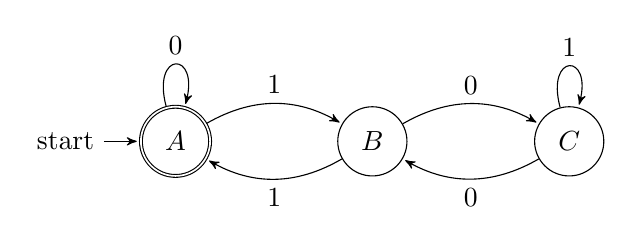
\begin{tikzpicture}[>=stealth',shorten >=1pt,auto,node distance=2.5cm]

    \node[initial,state,accepting] (A)              {$A$};
    \node[state]                   (B) [right of=A] {$B$};
    \node[state]                   (C) [right of=B] {$C$};

    \path[->] (A) edge [loop above] node {0} (A);
    \path[->] (A) edge [bend left]  node {1} (B);
    \path[->] (B) edge [bend left]  node {1} (A);
    \path[->] (B) edge [bend left]  node {0} (C);
    \path[->] (C) edge [bend left]  node {0} (B);
    \path[->] (C) edge [loop above] node {1} (C);

  \end{tikzpicture} \\
  Is the finite state diagram for this machine were $A = 0 \, \text{mod} \, n
  $, $B = 1 \, \text{mod} \, n$ and $C = 2 \, \text{mod} \, n$.

\section{Nondeterministic Finite Automata}
  \begin{itemize}
    \item A nondeterministic finite automaton (NFA) consists of
      \begin{itemize}
        \item A finite set of states $Q$.
        \item An input alphabet consisting of a finite set of symbols
        $\Sigma$.
        \item A transition function $\delta$ that maps $Q \times \Sigma$ to
        $P(Q)$, the set of subsets of $Q$. \\
        Like a DFA, this transition function can be represented by a
        transition diagram in which the nodes are labeled by states and arcs
        by symbols. Unlike a DFA, an NFA may have transitions to zero or more
        states from a given state on a given input symbol.
        \item A start state that is one of the states in $Q$.
        \item A set of final (or accepting) states $F$ that is a subset of
        $Q$.
      \end{itemize}
    \item An NFA accepts an input string $x$ if there is a path of transitions
    from the initial state to a final state that spells out $x$. Note that,
    unlike for a DFA, in an NFA, there may be more than one path from the
    initial state to a final state that spells out $x$.
    \item Note the definition of an extended transition function for an NFA.
    See Sect 2.3.3 of HMU.
    \item $L(A)$, the language defined by an NFA $N$ is the set of string
    accepted by $N$.
  \end{itemize}
  NP vs P? Nondeterministic Polynomial time vs Polynomial time.\\
  $L = \{\, w \, | \, w$ is a string of \texttt{a}'s and \texttt{b}'s ending
  in \texttt{abb} \} \\
  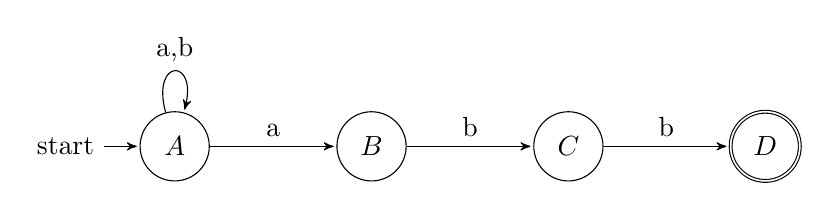
\begin{tikzpicture}[>=stealth',shorten >=1pt,auto,node distance=2.5cm]

    \node[initial,state]   (A)              {$A$};
    \node[state]           (B) [right of=A] {$B$};
    \node[state]           (C) [right of=B] {$C$};
    \node[state,accepting] (D) [right of=C] {$D$};

    \path[->] (A) edge [loop above] node {a,b} (A);
    \path[->] (A) edge              node {a}   (B);
    \path[->] (B) edge              node {b}   (C);
    \path[->] (C) edge              node {b}   (D);

  \end{tikzpicture} \\
  A nondeterministic machine is omniscient.

\section{Equivalence of DFAs and NFAs: the Subset Construction}
  \begin{itemize}
    \item From an NFA $N = (Q_N, \Sigma, \delta_N, q_0, F_N)$, we can
    construct a DFA $D = (Q_D, \Sigma, \delta_D, \{q_0\}, F_D)$ that simulates
    all possible moves of $N$ on any given input as follows:
      \begin{itemize}
        \item $Q_D$ is the set of all subsets of $Q_N$.
        \item The input alphabet of $D$ is the same as that of $N$.
        \item For each state $S$ in $Q_N$ and each input symbol \texttt{a} in
        $\Sigma$. \\
        $\delta_D(S, \texttt{a})$ is the union of all states in $\delta_N(
        \texttt{p}, \texttt{a})$ for all \texttt{p} in $S$.
        \item The start state of $D$ is the state \{ $\texttt{q}_0$ \}.
        \item $F_D$, the final states of $D$, are those states of $Q_D$ that
        contains a state in $F_N$.
      \end{itemize}
    \item We can prove by induction on the length of an input string
    \texttt{w}
    that $D$ can reach deterministic state $S$ in $Q_D$ on \texttt{w} iff $N$
    can reach each nondeterministic state \texttt{p} in $S$ on \texttt{w}. See
    Sect. 2.3.5 of HMU.
  \end{itemize}
  For the example of last section: \\
    \begin{tabular}{c|c c }
       State             & a                 & b                 \\ \hline
       \texttt{\{A\}}    & \texttt{\{A, B\}} & \texttt{\{A\}}    \\
       \texttt{\{A, B\}} & \texttt{\{A, B\}} & \texttt{\{A, C\}} \\
       \texttt{\{A, C\}} & \texttt{\{A, B\}} & \texttt{\{A, D\}} \\
       \texttt{\{A, D\}} & \texttt{\{A, B\}} & \texttt{\{A\}}    \\
    \end{tabular}


\section{Bad Case for the Subset Construction}
  \begin{itemize}
    \item Let $L$ be the language $(a + b)*a(a+b)^{n-1}$, that is, all strings
    of a's and b's in which the $n^{th}$ character from the end is an ``a''.
    The smallest DFA that accepts $L$ must have at least $2^n$ states.
  \end{itemize}
  We have an NFA $N$ that we want to transform into a DFA $D$ such that
  $L(N) = L(D)$. Thus, the states on the DFA are going to be subsets of the
  states used in the NFA.

\section{Practice Problems}
  \begin{enumerate}
    \item Let $L$ be the language \{ \texttt{w | w} is any string of
    \texttt{a}'s and \texttt{b}'s containing at least one \texttt{a} and at
    least one \texttt{b} \}.
      \begin{enumerate}
        \item Construct a DFA for $L$.
        \item Show the behavior of your DFA processing the input string
        \texttt{aabaa}.
      \end{enumerate}
    \item Let $L$ be the language \{ \texttt{abxba | x} is any string of
    \texttt{a}'s, \texttt{b}'s, and \texttt{c}'s not containing
    \texttt{ba} \}.
    This language models comments in the programming language C.
      \begin{enumerate}
        \item Construct a DFA for $L$.
        \item Show the behavior of your DFA processing the input string
        \texttt{abcbaba}.
      \end{enumerate}
    \item Let $L$ be the language consisting of all strings of \texttt{a}'s
    and \texttt{b}'s containing the substring \texttt{abba}. Construct a DFA
    for $L$.
    \item Let L be the language consisting of all strings of \texttt{0}'s and
    \texttt{1}'s having an even number of \texttt{0} and an even number of
    \texttt{1}'s.
      \begin{enumerate}
        \item Construct a DFA for $L$.
        \item Show the behavior of your DFA processing the input string
        \texttt{01100101}.
        \item Prove that your DFA is correct.
      \end{enumerate}
    \item Construct an NFA that accepts all strings of \texttt{a}'s and
    \texttt{b}'s ending in \texttt{abb}.
      \begin{enumerate}
        \item Show all sequences of moves that your NFA can make on the input
        string \texttt{ababb}
        \item Use the subset construction to convert your NFA into an
        equivalent DFA.
      \end{enumerate}
    \item Construct an NFA that accepts all strings of \texttt{a}'s and
    \texttt{b}'s in which the third last character is an \texttt{a}.
      \begin{enumerate}
        \item Use the subset construction to convert your NFA into an
        equivalent DFA.
        \item Prove that any DFA recognizing this language must have at least
        eight states.
      \end{enumerate}
  \end{enumerate}

\section{Reading Assignment}
  \begin{itemize}
    \item HMU: Ch. 2
  \end{itemize}

\end{document}
